\documentclass[10pt,a4paper]{amsart}
\usepackage[margin=19mm]{geometry}
\usepackage{amsmath,amssymb,mathtools}
\usepackage[scr=rsfs,cal=euler]{mathalfa}
\usepackage{xfrac}
\usepackage[unicode,hidelinks,bookmarks=false]{hyperref}
\newcommand{\ie}{i.e.\ }
\newcommand{\cf}{cf.\ }
\newcommand{\resp}{respectively\ }
\newcommand{\Subsection}{\subsection}
\providecommand{\nobreakdash}{\nobreak\hbox{-}}
\setlength{\emergencystretch}{2em}
\multlinegap0pt
\usepackage{tikz}
\newtheorem{definition}{Definition}
\newtheorem{theorem}{Theorem}
\newtheorem{lemma}{Lemma}
\newcommand{\id}{\mathrm{id}}
\title{The Brauer category $\mathcal{B}(2)$ has \\ principal graph $D_\infty$}
\author{Stephen Bigelow}
\date{Source: arXiv:2608.18328v1 (CC BY 4.0)}
\begin{document}
\maketitle

\noindent\emph{Source and licence.} The Brauer category $\mathcal{B}(2)$ has \\ principal graph $D_\infty$. Version arXiv:2608.18328v1 (CC BY 4.0), distributed by arXiv under the Creative Commons Attribution 4.0 International licence, http://creativecommons.org/licenses/by/4.0/, as recorded in the arXiv licence metadata for this exact version and shown on the abstract page https://arxiv.org/abs/2608.18328v1. Full licence notice: \texttt{licenses/arxiv-2608.18328-CC-BY-4.0.txt}.\par\smallskip

\noindent\textit{Editorial scope.} Counted unit: the article's theorem thm:principal (source0.tex lines 264--269). The article's complete original proof of it is delivered with it (source0.tex lines 599--721, one \texttt{proof} environment of 123 lines, which the article places away from the statement). No mathematics is written, repaired or re-derived: the statement and the proof are the article's own lines, in the article's own notation, and no retained line is substituted or re-flowed.  Retained uncounted as the source-local context the proof needs: lines 250--258; lines 577--581.  Nothing was omitted from any retained span, so the package carries no omission record.  No retained line contains a citation, so the wrapper carries no bibliography and no bibliography entry.  The retained lines contain the article's own diagram code, which the wrapper typesets with the standard tikz packages; no image file is delivered and the package declares no asset dependency.  Editorial formatting only, in addition: an AMS \texttt{amsart} preamble that restates the article's own declarations and macros used by the retained lines, namely the environments \texttt{definition}, \texttt{theorem}, \texttt{lemma} on separate counters, together with the standard packages those lines need.  The retained environments print in this document as Definition 1, Theorem 1, Lemma 1 in order of appearance, whereas the article prints the same items with the numbering of its own full document.  The complete native source of the article as distributed in the arXiv e-print for this exact version is bundled unchanged as \texttt{sources/207983/source0.tex}.
\begin{definition}
\label{def:principal}
Let $\mathcal{C}$ and $\Gamma$ be as above.  We say $\mathcal{C}$
has \emph{principal graph} $\Gamma$ if we can assign a brick $P_v$
to each vertex $v$ such that the $P_v$ are pairwise orthogonal, if $v$
is the base vertex then $P_v=\id_0$, and every $P_v \otimes \id_1$ is
isomorphic to the direct sum of $P_w$ over all vertices $w$ adjacent to
$v$ in $\Gamma$.
\end{definition}

\begin{lemma}
\label{lem:uniqueuptoscalar}
If $Q$ is an uncappable $n$-box that can eat a crossing at its top left
then $Q$ is a scalar multiple of $P_n$.
\end{lemma}

\begin{theorem}
\label{thm:principal}
The reduced Brauer category $\overline{\mathcal{B}}$ at
$\delta=2$ has principal graph $D_\infty$, in the sense of
Definition~\ref{def:principal}.
\end{theorem}

\begin{proof}[Proof of Theorem \ref{thm:principal}]
We must show that each $P_v$ is in fact an idempotent.  In $P_v^2$, expand
out the top copy of $P_v$, and use the fact that the bottom copy of $P_v$
is uncappable and eats crossings.  The result is $P_v$ in every case.

We also have to check that $P_v$ is non-zero and not a torsion element.
An easy way to do this is to calculate the trace of $P_v$.  This is $1$
for $P_0$ and $P_{2'}$, and $2$ for $P_1,P_2,P_3,\dots$.

Now we show that every morphism of the form $P_vfP_v$ is a scalar
multiple of $P_v$.  We can assume $f$ is a single Brauer diagram.
Let each $P_v$ eat crossings.  Either we reduce to a diagram with a cup
or cap, or the identity diagram.  The result is zero, or $P_v^2=P_v$,
or $-P_v$ if $v=2'$ and $f$ was a single crossing.

A similar argument can be used to show that every morphism of the form
$P_wfP_v$ is zero when $v \neq w$.  Eat crossings and reduce to a diagram
with a cup or cap, or the identity diagram.  A cup or cap gives zero.
The identity diagram can only happen when $P_v$ and $P_w$ are in the
same $n$-box space, in which case we have
$$P_2 P_{2'} = P_{2'} P_2 = 0.$$

It remains to show that show that, for all $v$, $P_v \otimes \id_1$
is isomorphic to the direct sum of $P_w$ over all $w$ adjacent to $v$.

For $v=0$, we have $P_0 \otimes \id_1 = P_1$.
For $v=1$, we have $P_1 \otimes \mathrm{id}_1 = P_2 + P_{2'} + E$,
where $E$ is the Jones idempotent
$$
E=
\frac12\;

\begin{tikzpicture}[baseline=-0.5ex,scale=0.05]
\draw (-5,-5) .. controls (-5,0) and (5,0) .. (5,-5);
\draw (-5,5) .. controls (-5,0) and (5,0) .. (5,5);
\end{tikzpicture}
\simeq
\frac12\;

\begin{tikzpicture}[baseline=-0.5ex,scale=0.05]
\draw (-5,0) .. controls (-5,5) and (5,5) .. (5,0)
             .. controls (5,-5) and (-5,-5) .. (-5,0);
\end{tikzpicture}
= P_0.
$$
For $v=2'$, the leaf relation implies
\[
P_{2'} \otimes \mathrm{id}_1
=2\;
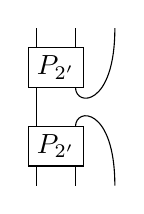
\begin{tikzpicture}[baseline=-0.5ex,scale=0.05]
\node at (-5,10) {$P_{2'}$};
\draw (-12,5) rectangle (2,15);
\node at (-5,-10) {$P_{2'}$};
\draw (-12,-15) rectangle (2,-5);
\draw (-10,-20) -- (-10,-15);
\draw (-10,-5) -- (-10,5);
\draw (-10,15) -- (-10,20);
\draw (0,-20) -- (0,-15);
\draw (0,-5) .. controls (0,0) and (10,0) .. (10,-20);
\draw (0,5) .. controls (0,0) and (10,0) .. (10,20);
\draw (0,15) -- (0,20);
\end{tikzpicture}
\simeq
2\;
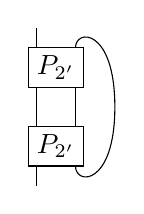
\begin{tikzpicture}[baseline=-0.5ex,scale=0.05]
\node at (-5,10) {$P_{2'}$};
\draw (-12,5) rectangle (2,15);
\node at (-5,-10) {$P_{2'}$};
\draw (-12,-15) rectangle (2,-5);
\draw (-10,-20) -- (-10,-15);
\draw (-10,-5) -- (-10,5);
\draw (-10,15) -- (-10,20);
\draw (0,-15) .. controls (0,-20) and (10,-20) .. (10,0)
              .. controls (10,20) and (0,20) .. (0,15);
\draw (0,-5) -- (0,5);
\end{tikzpicture}
=P_1.
\]
Finally, for $v=2,3,\dots$, I claim we have
$$P_v \otimes \mathrm{id}_1 = P_{v+1} + F,$$
where $F$ is as follows.
\[
F=
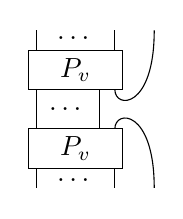
\begin{tikzpicture}[baseline=-0.5ex,scale=0.05]
\node at (-10,10) {$P_v$};
\draw (-22,5) rectangle (2,15);
\node at (-10,-10) {$P_v$};
\draw (-22,-15) rectangle (2,-5);
\draw (-20,-5) -- (-20,5);
\node at (-12,0) {$\dots$};
\draw (-4,-5) -- (-4,5);
\draw (0,-5) .. controls (0,0) and (10,0) .. (10,-20);
\draw (0,5) .. controls (0,0) and (10,0) .. (10,20);
\draw (-20,-20) -- (-20,-15);
\node at (-10,-18) {$\dots$};
\draw (0,-20) -- (0,-15);
\draw (-20,15) -- (-20,20);
\node at (-10,18) {$\dots$};
\draw (0,15) -- (0,20);
\end{tikzpicture}
\simeq
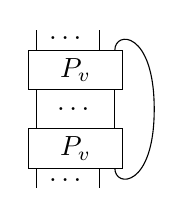
\begin{tikzpicture}[baseline=-0.5ex,scale=0.05]
\node at (-10,10) {$P_v$};
\draw (-22,5) rectangle (2,15);
\node at (-10,-10) {$P_v$};
\draw (-22,-15) rectangle (2,-5);
\draw (-20,-5) -- (-20,5);
\node at (-10,0) {$\dots$};
\draw (0,-5) -- (0,5);
\draw (0,-15) .. controls (0,-20) and (10,-20) .. (10,0)
              .. controls (10,20) and (0,20) .. (0,15);
\draw (-20,-20) -- (-20,-15);
\node at (-12,-18) {$\dots$};
\draw (-4,-20) -- (-4,-15);
\draw (-20,15) -- (-20,20);
\node at (-12,18) {$\dots$};
\draw (-4,15) -- (-4,20);
\end{tikzpicture}
= P_{v-1}.
\]
Here, $P_v\otimes\id_1-F=P_{v+1}$ holds up to a scalar by
Lemma~\ref{lem:uniqueuptoscalar}.  An easy way to check that the scalar
is $1$ is to calculate traces, which are $2$ for $P_{v+1}$ and $P_v$,
and $4$ for $P_v\otimes\id_1$.
\end{proof}

\end{document}
